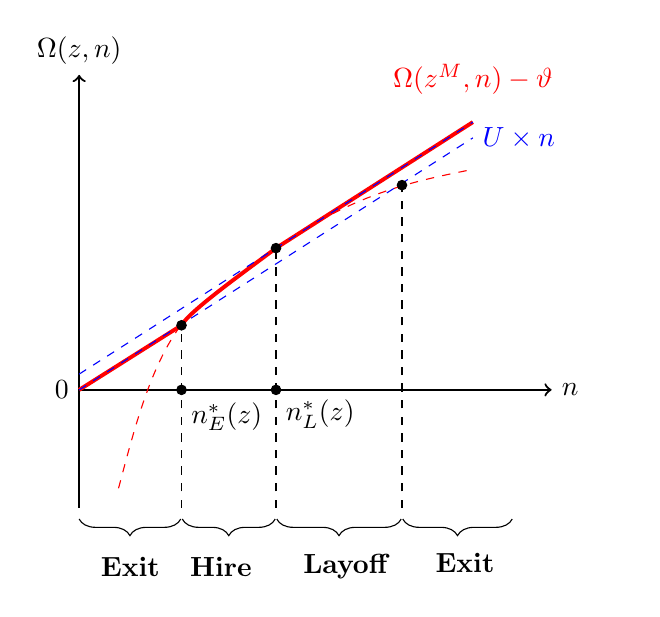
\begin{tikzpicture}

% Axes
\draw[thick,->] (0,0)--(0,5.5) node[above]{$\Omega(z,n)$};
\draw[thick,->] (0,1.5) node[left]{$0$} --(6,1.5) node[right]{$n$};

% Omega
\draw[dashed,red] (0.5,0.25) ..controls (0.7,1) and (0.9,1.8) .. (1.3,2.332);
\draw[dashed,red] (2.5,3.3) ..controls (3.5,4) and (4.25,4.15) .. (5,4.3);

\draw[line width = 0.5mm,red] (0,1.5)--(1.3,2.32);
\draw[line width = 0.5mm,red] (1.3,2.32) ..controls (1.4,2.5) and (2.1,3) .. (2.5,3.3);
\draw[line width = 0.5mm,red] (2.5,3.3)--(5,4.9) node[above,yshift=6pt]{$\pmb{\Omega(z^M,n)-\vartheta}$};

% U n
\draw[dashed,blue](0,1.5)--(5,4.7) node[right]{$U \times n$};
\draw[dashed,blue](0,1.7)--(5,4.9) node[right]{\hskip17.8mm \ };

% Dots
\draw[fill] (1.3,2.32) circle [radius=0.06];
\draw[fill] (2.5,3.3) circle [radius=0.06];
\draw[fill] (4.1,4.1) circle [radius=0.06];

% Dashed lines
\draw[dashed] (1.3,0)--(1.3,2.32)node[right,yshift=-33pt]{$n_E^\ast(z)$};
\draw[fill]   (1.3,1.5) circle [radius=0.06];
\draw[dashed] (2.5,0) --(2.5,3.3)node[right,yshift=-60pt]{$n_L^\ast(z)$};
\draw[fill]   (2.5,1.5) circle [radius=0.06];
\draw[dashed] (4.1,0) --(4.1,4.1);

% Braces
\draw[decorate, decoration = {brace, amplitude = 6pt,mirror}, xshift = 0pt, yshift = -4pt] (0, 0) -- (1.29, 0);
\draw (0.65,-0.75) node{\textbf{\alertroyalblue{Exit}}};

\draw[decorate, decoration = {brace, amplitude = 6pt,mirror}, xshift = 0pt, yshift = -4pt] (1.31, 0) -- (2.49, 0);
\draw (1.8,-0.75) node{\textbf{\alert{Hire}}};

\draw[decorate, decoration = {brace, amplitude = 6pt,mirror}, xshift = 0pt, yshift = -4pt] (2.51, 0) -- (4.09, 0);
\draw (3.4,-0.75) node{\textbf{\alertroyalblue{Layoff}}};

\draw[decorate, decoration = {brace, amplitude = 6pt,mirror}, xshift = 0pt, yshift = -4pt] (4.11, 0) -- (5.5, 0);
\draw (4.9,-0.7) node{\textbf{\alertroyalblue{Exit}}};

\end{tikzpicture}
